   	\newpage   	
   	\section{Projektplanung}
   	Die zu entwickelnde Android Applikation LIAR ist ein Gesellschaftsspiel auf Basis eines Lügendetektors. Die Applikation soll es ermöglichen, ein Nutzer A einem anderen Nutzer B Fragen stellt, welcher dieser beantwortet. Dabei wird mittels eines EEG-Sensors und mit Hilfe eines Galvanic Skin Sensors die Anspannung des Nutzers evaluiert. Im Anschluss erlaubt die LIAR App eines Aussage zum Wahrheitsgehalt der Antwort des Nutzers.
   	
   	\newpage
   	\subsection{Meilensteine}
	Meilensteine repräsentieren Zwischenergebnisse in der Programmentwicklung die von besonderer Bedeutung sind. Sie eignen sich zur Arbeitsaufteilung in einer Gruppe.
	\subsubsection{Einarbeitung}
	\begin{itemize}
	\item{}Android SDK installieren
	\item{}Android Tutorial absolvieren
	\item{}Einarbeitung in Mindwave Mobile (EEG-Sensor)
	\item{}Einarbeitung in das SDK des Galvanic Skin Sensors
	\end{itemize}	  	
	\subsubsection{Aufbau eines User Interfaces}
	\begin{itemize}
	\item{}Hauptbildschirm mit den Elementen(neues Spiel starten, Eigenanalyse, Ranglisten und Spielanleitung)
	\item{}Spielstartbildschirm auf dem die Anzahl der zu spielenden Runden, die Anzahl der Spieler und deren Namen eingetragen werden können.
	\item{}Eigenanalysebildschirm: zeigt die Messwerte beider Sensoren in zwei Graphen an und erlaubt eine Aufzeichnung von Daten, eine Ansicht älterer Daten, sowie zwei Informationsbuttons mit Wissenswerten Informationen zum EEG und Galvanic Skin Sensor
	\item{}Auswertungsbildschirm: zeigt das Ergebnis der Fragerunde (Anzahl der wahrheitsgemäß beantworteten Fragen, Anzahl der vermeintlich nicht wahrheitsgemäß beantworteten Fragen, Batch-System für das Erreichen einer besonderen Leistung [z.B. ehrliche Haut oder Lügner des Monats]) und ermöglicht das Teilen des Ergebnisses auf Facebook
	\end{itemize}
	\subsubsection{Anbindung des EEG Sensors}
	\begin{itemize}
	\item{}Einrichtung einer Bluetoothverbindung zum EEG-Sensor
	\item{}Auslesen der Daten des EEG-Sensors
	\item{}Interpretieren der Daten des EEG-Sensors
	\item{}grafische Darstellung der Daten des EEG-Sensors
	\end{itemize}
	\subsubsection{Anbindung des Galvanic Skin Sensors}
	\begin{itemize}
	\item{}Einrichtung einer Bluetoothverbindung vom Arduino Shield zum Galvanic Skin Sensor
	\item{}Einrichtung einer Bluetoothverbindung vom Smartphone zum Arduino Shield
	\item{}Auslesen der Daten der Messdaten
	\item{}Interpretieren der Messdaten
	\item{}grafische Darstellung der Messdaten
	\end{itemize}
   	

	\newpage
   	\subsection{fiktive Zeitungsmeldung}
   	Die folgende fiktive Zeitungsmeldung stellt aus Sicht der Entwickler die Perspektiven und Erwartungen an das LIAR Projekt dar. 
	\begin{figure}[ht!]
		\begin{center}
			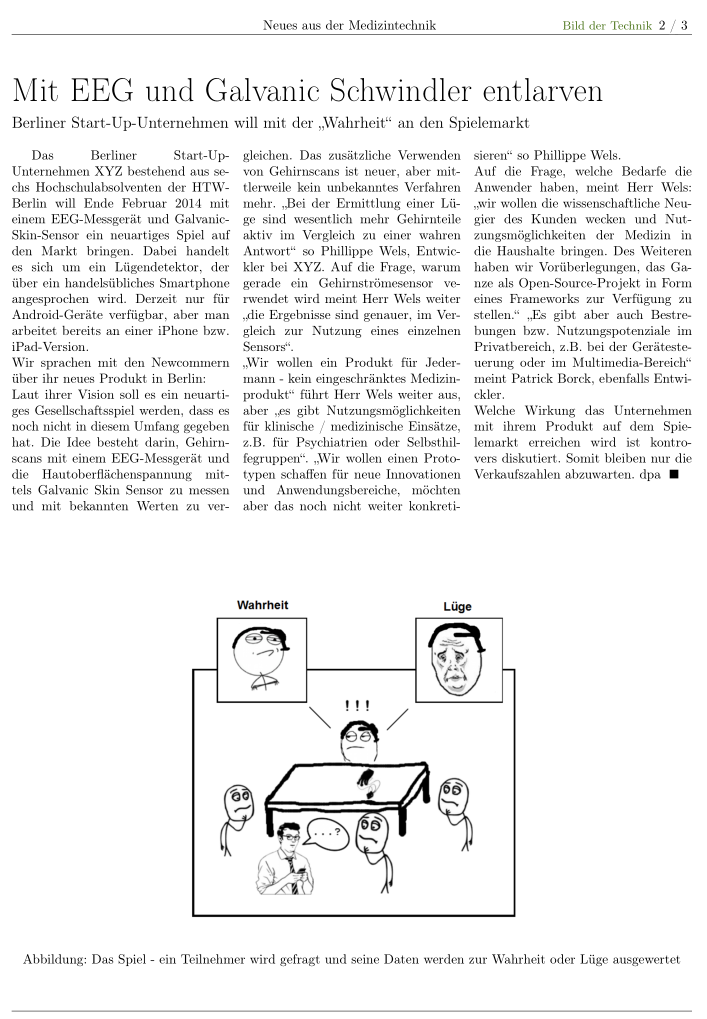
\includegraphics[width=0.8\textwidth]{zeitungsmeldung.png}
		\end{center}
		\caption[Zeitungsmeldung]{fiktive Zeitungsmeldung}
	\label{fig:zeitungsmeldung}
	\end{figure}   

	%\includepdf[pagecommand={\thispagestyle{fancy}}, pages=2, scale=0.55, frame=true]{pdf/zeitungsmeldung.pdf}   

   	\subsection{Produktverpackung}
   	Die folgende Abbildung stellt die auf die Nutzergruppe angepasste Produktverpackung der LIAR-App dar.
	\begin{figure}[ht!]
	\begin{center}
		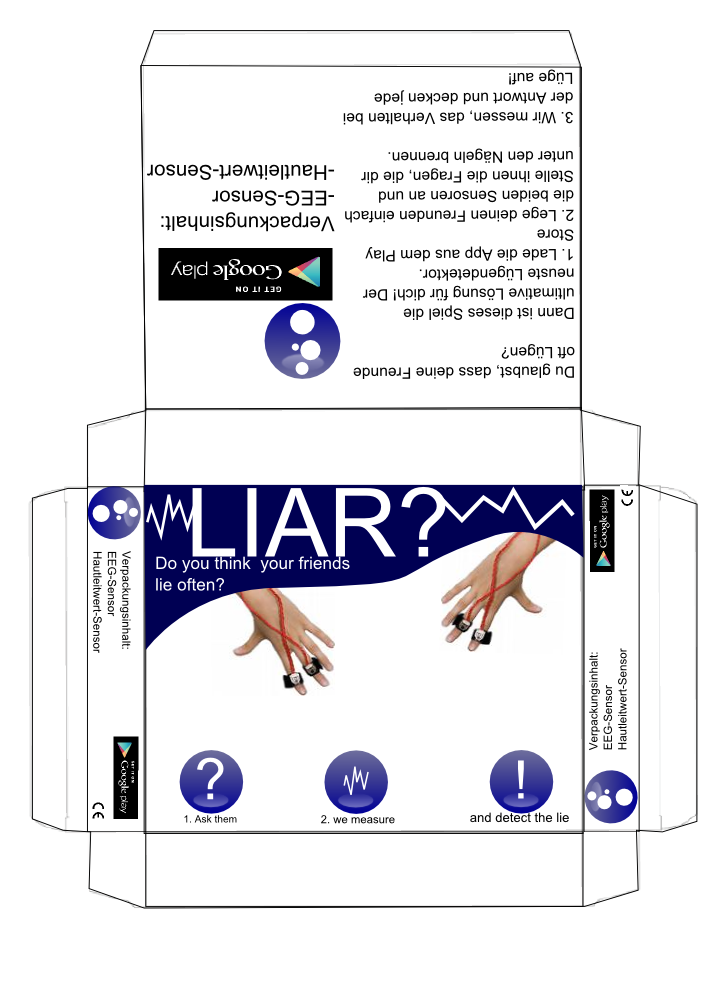
\includegraphics[width=0.8\textwidth]{verpackung.png}
	\end{center}
	\caption[Produktverpackung]{Produktverpackung Liar Android App}
	\label{fig:verpackung}
	\end{figure}   
